\let\negmedspace\undefined
\let\negthickspace\undefined
\documentclass[journal]{IEEEtran}
\usepackage[a5paper, margin=10mm, onecolumn]{geometry}
%\usepackage{lmodern} % Ensure lmodern is loaded for pdflatex
\usepackage{tfrupee} % Include tfrupee package

\setlength{\headheight}{1cm} % Set the height of the header box
\setlength{\headsep}{0mm}     % Set the distance between the header box and the top of the text

\usepackage{gvv-book}
\usepackage{gvv}
\usepackage{cite}
\usepackage{amsmath,amssymb,amsfonts,amsthm}
\usepackage{algorithmic}
\usepackage{graphicx}
\usepackage{textcomp}
\usepackage{xcolor}
\usepackage{txfonts}
\usepackage{listings}
\usepackage{enumitem}
\usepackage{mathtools}
\usepackage{gensymb}
\usepackage{comment}
%\usepackage{multiclo}
\usepackage[breaklinks=true]{hyperref}
\usepackage{tkz-euclide} 
\usepackage{listings}
% \usepackage{gvv} 
\graphicspath{ {./figs/} }

\begin{document}

\title{
AR: ARCHITECTURE AND PLANNING}
\author{AI25BTECH11011}
\maketitle
\renewcommand{\thefigure}{\theenumi}
\renewcommand{\thetable}{\theenumi}

\begin{enumerate}

\item Natural granite used for cladding in buildings belongs to the category of
\begin{multicols}{4}
\begin{enumerate}
\item Igneous Rock
\item Acid Rock
\item Sedimentary Rock
\item Metamorphic Rock
\end{enumerate}
\end{multicols}
\hfill (GATE AR 2010)

\item 'Flying Buttress' is an architectural element of
\begin{multicols}{2}
\begin{enumerate}
\item Indian Architecture
\item Greek Architecture
\item Gothic Architecture
\item Byzantine Architecture
\end{enumerate}
\end{multicols}
\hfill (GATE AR 2010)

\item A major hole in the Ozone layer has been identified above the
\begin{multicols}{2}
\begin{enumerate}
\item Amazon Forest
\item Arctic Region
\item Savannah Grasslands
\item Sahara Desert
\end{enumerate}
\end{multicols}
\hfill (GATE AR 2010)

\item A flat arch at the skewback should NOT have an angle less than
\begin{multicols}{4}
\begin{enumerate}
\item $30^\circ$
\item $45^\circ$
\item $60^\circ$
\item $90^\circ$
\end{enumerate}
\end{multicols}
\hfill (GATE AR 2010)

\item Primary colours of natural light are
\begin{multicols}{2}
\begin{enumerate}
\item Red, Blue, Yellow
\item Red, Green, Blue
\item Red, Violet, Yellow
\item Red, Green, Yellow
\end{enumerate}
\end{multicols}
\hfill (GATE AR 2010)

\item Horizontal member of a shutter that subdivides a window is termed as
\begin{multicols}{4}
\begin{enumerate}
\item Mullion
\item Transorn
\item Reveal
\item Purlin
\end{enumerate}
\end{multicols}
\hfill (GATE AR 2010)

\item If the temperature of a composite bar made of copper and steel is raised, then the copper bar will be under
\begin{multicols}{4}
\begin{enumerate}
\item Tension
\item Compression
\item Shear
\item Torsion
\end{enumerate}
\end{multicols}
\hfill (GATE AR 2010)

\item E.I.A. stands for
\begin{multicols}{2}
\begin{enumerate}
\item East India Association
\item Environmental Impact Audit
\item Environment Impact in Asia
\item Environmental Impact Assessment
\end{enumerate}
\end{multicols}
\hfill (GATE AR 2010)

\item A steel truss with parallel upper and lower chords and inclined connecting members forming a series of equilateral triangles is known as
\begin{multicols}{2}
\begin{enumerate}
\item Bowsiring Truss
\item Warren Truss
\item Kingpost Truss
\item Scissors Truss
\end{enumerate}
\end{multicols}
\hfill (GATE AR 2010)

\item In water supply systems, the 'Reflux Valves' allow water to flow
\begin{multicols}{2}
\begin{enumerate}
\item In one direction only
\item In both directions
\item Through air locked joints
\item Only under low pressure
\end{enumerate}
\end{multicols}
\hfill (GATE AR 2010)

\item In Islamic Architecture, the circular dome was constructed over a square configuration through
\begin{enumerate}
\item Grid Iron Coffered Slab
\item Pendentives and Squinch Arches
\item Double Barrel Vaulis and Jack Arches
\item Horizontal Cross Tie Members
\end{enumerate}
\hfill (GATE AR 2010)

\item With respect to energy conservation and cost efficiency, the nature of an ideal built form should be
\begin{multicols}{2}
\begin{enumerate}
\item High Rise Low Density
\item Medium Rise High Density
\item Low Rise High Density
\item Low Rise Low Density
\end{enumerate}
\end{multicols}
\hfill (GATE AR 2010)

\item Two default sequences P and Q are given below :

P: Specify height of extrusion or [Path]: 50

Specify angle of taper for extrusion $<0>$:

Q: Specify height of extrusion or [Path]: p

Select extrusion path or [Taper angle]:

The above mentioned sequences P and Q respectively, belong to
\begin{multicols}{2}
\begin{enumerate}
\item 2D AutoCAD and 2D AutoCAD
\item 2D and 3D AutoCAD
\item 3D and 2D AutoCAD
\item 3D AutoCAD and 3D AutoCAD
\end{enumerate}
\end{multicols}
\hfill (GATE AR 2010)

\item When shear stress exceeds the permissible limit in a RCC slab, then this problem is solved by
\begin{multicols}{2}
\begin{enumerate}
\item Increasing the slab depth
\item Providing shear reinforcement
\item Using high strength steel
\item Using thinner bars but more in number
\end{enumerate}
\end{multicols}
\hfill (GATE AR 2010)

\item Considering the total heat losses from all fluorescent lamps to be 79\%, the Heating load (Btu / hr) due to office illumination with 48 ceiling mounted luminaires, each containing four 40 W fluorescent lamps and flat surface diffusers will be
\begin{multicols}{2}
\begin{enumerate}
\item 10000 Btu / hr
\item 15000 Btu / hr
\item 17500 Btu / hr
\item 21000 Btu / hr
\end{enumerate}
\end{multicols}
\hfill (GATE AR 2010)

\item Prime resultant forces that develop in a structure due to an earthquake depend on
\begin{enumerate}
\item Mass and Surface Area of structure
\item Surface Area and Stiffness of structure
\item Stiffness and Mass of structure
\item Surface Area and Volume of structure
\end{enumerate}
\hfill (GATE AR 2010)

\item Concept of 'Serial Vision' has been applied to the approach layout of
\begin{multicols}{2}
\begin{enumerate}
\item Victoria Memorial Complex, Kolkata
\item Umaid Bhawan Palace, Jodhpur
\item Vidhan Soudha Precinct, Bangalore
\item Rashtrapati Bhawan Complex, New Delhi
\end{enumerate}
\end{multicols}
\hfill (GATE AR 2010)

\item Advanced Traffic Lane Information is an important feature of
\begin{multicols}{2}
\begin{enumerate}
\item Para Transit system
\item Intelligent Transportation system
\item High Level Cable Car system
\item Pedestrian Travellator system
\end{enumerate}
\end{multicols}
\hfill (GATE AR 2010)

\item A local authority can go for Urban Development through
\begin{multicols}{2}
\begin{enumerate}
\item Land Acquisition
\item Land Pooling
\item Transferable Development Rights
\item All the above
\end{enumerate}
\end{multicols}
\hfill (GATE AR 2010)

\item The Planning document submitted for the selected cities under JNNURM is
\begin{multicols}{2}
\begin{enumerate}
\item Master Plan
\item Basic Development Plan
\item City Development Plan
\item Outline Development Plan
\end{enumerate}
\end{multicols}
\hfill (GATE AR 2010)

\item Excessive tilt of the Leaning Tower of Pisa has been checked by
\begin{enumerate}
\item Pumping cement concrete mix under the dipping foundation
\item Relocating heavier furniture to the rising side of the tower
\item Raising the dipping side by massive Jack screws
\item Pumping out mud and slurry from the foundation base of the rising side
\end{enumerate}
\hfill (GATE AR 2010)

\item The Pritzker Prize 2009 has been awarded to
\begin{multicols}{2}
\begin{enumerate}
\item Zaha Hadid
\item Peter Zumthor
\item Jean Nouvel
\item Norman Foster
\end{enumerate}
\end{multicols}
\hfill (GATE AR 2010)

\item The age of a tree is determined by
\begin{enumerate}
\item Counting the number of rings in the stem cross section
\item Counting the number of leaves on the main branches
\item Measuring the height of the tree from the rootball
\item Measuring the canopy circumference of the tree
\end{enumerate}
\hfill (GATE AR 2010)

\item Nakagin Capsule Tower, Tokyo famous for its spatial modular approach was designed by
\begin{multicols}{2}
\begin{enumerate}
\item Arata Isozaki
\item Tadao Ando
\item Kisho Kurokawa
\item Minoru Yamasaki
\end{enumerate}
\end{multicols}
\hfill (GATE AR 2010)

\item Proportioning system used in the layout of Mughal Gardens is derived from
\begin{enumerate}
\item Rational number system
\item Constants of equilateral triangle
\item Irrational number system
\item Constants of right angled isosceles triangle
\end{enumerate}
\hfill (GATE AR 2010)

\item Match the cities in Group I with their form in Group II

\begin{table}[H]
\centering
\begin{tabular}{cc}
\textbf{Group I} & \textbf{Group II} \\
P. Detroit & 1. Star Form \\
Q. Copenhagen & 2. Polycentred Net \\
R. Stalingrad & 3. Linear City \\
S. San Francisco & 4. Ring Form \\
& 5. Galaxy \\
\end{tabular}
\end{table}

\begin{multicols}{2}
\begin{enumerate}
\item P - 1, Q - 4, R - 3, S - 2
\item P - 2, Q - 1, R - 3, S - 4
\item P - 5, Q - 1, R - 2, S - 3
\item P - 4, Q - 3, R - 1, S - 5
\end{enumerate}
\end{multicols}
\hfill (GATE AR 2010)

\item Match the visionaries in Group I with their concepts in Group II

\begin{table}[H]
\centering
\begin{tabular}{cc}
\textbf{Group I} & \textbf{Group II} \\
P. Clarence A. Perry & 1. Post Modernism \\
Q. Constantinos Doxiadis & 2. Bauhaus \\
R. Paul Davidoff & 3. Advocacy Planning \\
S. Walter Gropius & 4. Dynopolis \\
& 5. Neighborhood Unit \\
\end{tabular}
\end{table}

\begin{multicols}{2}
\begin{enumerate}
\item P - 5, Q - 4, R - 3, S - 2
\item P - 5, Q - 4, R - 2, S - 1
\item P - 1, Q - 3, R - 2, S - 1
\item P - 2, Q - 4, R - 2, S - 5
\end{enumerate}
\end{multicols}
\hfill (GATE AR 2010)

\item Match the trees in Group I with their botanical names in Group II

\begin{table}[H]
\centering
\begin{tabular}{cc}
\textbf{Group I} & \textbf{Group II} \\
P. Neem & 1. Cassia Fistula \\
Q. Amaltas & 2. Azadirachia Indica \\
R. Pipal & 3. Ficus Bengalensis \\
S. Asoka & 4. Ficus Religiosa \\
& 5. Saraca Indica \\
\end{tabular}
\end{table}

\begin{multicols}{2}
\begin{enumerate}
\item P - 1, Q - 2, R - 3, S - 4
\item P - 3, Q - 4, R - 5, S - 1
\item P - 2, Q - 1, R - 4, S - 5
\item P - 2, Q - 3, R - 5, S - 4
\end{enumerate}
\end{multicols}
\hfill (GATE AR 2010)

\item Following graphs represent the relationship between city size (in terms of population) on X-axis and area under residential use (in percent) on Y-axis. Identify the correct graph.
\begin{multicols}{2}
\begin{enumerate}
\item 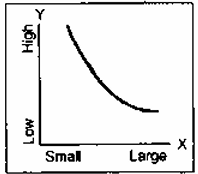
\includegraphics[width=0.2\textwidth]{Fig 1.png}
\item 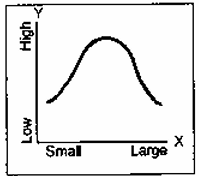
\includegraphics[width=0.2\textwidth]{Fig 2.png}
\item 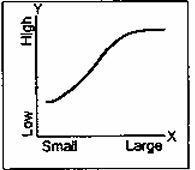
\includegraphics[width=0.2\textwidth]{Fig 3.png}
\item 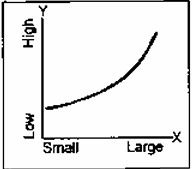
\includegraphics[width=0.2\textwidth]{Fig 4.png}
\end{enumerate}
\end{multicols}
\hfill (GATE AR 2010)

\item Global climate change is expected to bring about a combination of the following changes. Identify the correct combination.

P. Increase in Biodiversity

Q. Emergence of New Diseases

R. Loss of Biodiversity

S. Loss of all Rocky Outcrops

T. Sea Level Rise

U. Extinction of Polar Bears

V. Emergence of New Islands
\begin{multicols}{4}
\begin{enumerate}
\item P, Q, R, S
\item Q, R, T, U
\item R, T, U, V
\item Q, R, U, V
\end{enumerate}
\end{multicols}
\hfill (GATE AR 2010)

\item Annual housing demand of a metropolitan city is estimated through the combination of the following components. Identify the correct combination.

P. New Entrants to the City

Q. Elderly Population Living in Cities

R. New Relocated Slum Dwellers

S. Slum Squatter Dwellers

T. Unauthorized Dwelling Units

U. Dilapidated Houses

V. Part of Backlog

W. Any Other Houses
\begin{multicols}{4}
\begin{enumerate}
\item P, R, T
\item U, S, Q
\item W, Q, T
\item P, U, V
\end{enumerate}
\end{multicols}
\hfill (GATE AR 2010)

\item A square pin jointed truss is subjected to a load P, acting in the direction of member US, at joint U. The force in member UR is
\begin{figure}[H]
\centering
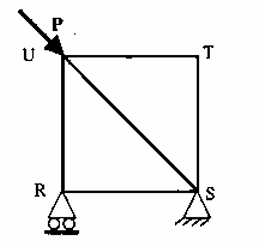
\includegraphics[width=0.4\textwidth]{Fig 5.png}
\caption{}
\label{fig:question32}
\end{figure}
\begin{multicols}{4}
\begin{enumerate}
\item 1.414 P
\item 1.000 P
\item 0.707 P
\item 0.000 P
\end{enumerate}
\end{multicols}
\hfill (GATE AR 2010)

\item Given below is the sketch plan of a site showing contours. The broken lines show valleys and ridges. Identify the ridges and valleys.
\begin{figure}[H]
\centering
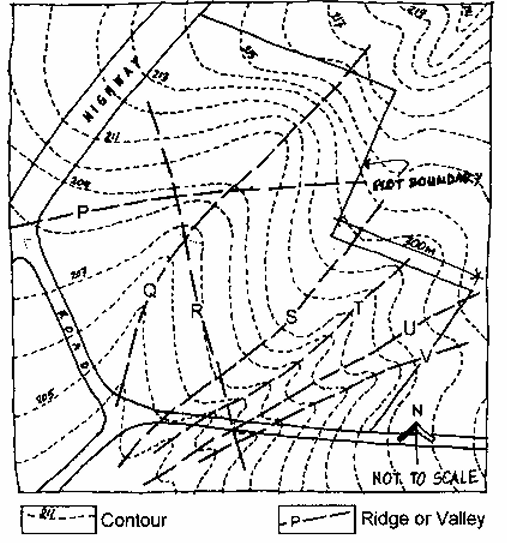
\includegraphics[width=0.5\textwidth]{Fig 6.png}
\caption{}
\label{fig:question33}
\end{figure}
\begin{multicols}{2}
\begin{enumerate}
\item Ridges: P, Q, R 

      Valleys: S, T
\item Ridges: T, V 

      Valleys: R, T, U
\item Ridges: S, U 

      Valleys: Q, T, V
\item Ridges: R, V, U 

      Valleys: P, T
\end{enumerate}
\end{multicols}
\hfill (GATE AR 2010)

\item From the following, identify the factors which influence the loudness of sound to a listener in an enclosure

P. Loudness of sound at source

Q. Directivity factor

R. Length/Width ratio of the enclosure

S. Distance between sound source and listener

U. Sound absorption co-efficient of all enclosing surfaces

V. Surface area of enclosing surfaces

Y. Inside temperature level of the enclosure
\begin{multicols}{4}
\begin{enumerate}
\item P, Q, S, Y, V
\item Q, R, S, U, Y
\item P, R, S, U, V
\item P, Q, S, U, V
\end{enumerate}
\end{multicols}
\hfill (GATE AR 2010)

\item Match the lamps in Group I with their Colour Rendering Index (CRI) in Group II

\begin{table}[H]
\centering
\begin{tabular}{cc}
\textbf{Group I} & \textbf{Group II} \\
P. Mercury Vapour & 1.65 - 70 \\
Q. Metal Halide & 2.40 - 55 \\
R. High-pressure sodium & 3.20 - 25 \\
S. Low-pressure sodium & 4.60 - 64 \\
\end{tabular}
\end{table}

\begin{multicols}{2}
\begin{enumerate}
\item P - 4, Q - 2, R - 1, S - 3
\item P - 3, Q - 2, R - 4, S - 1
\item P - 2, Q - 1, R - 4, S - 3
\item P - 4, Q - 3, R - 2, S - 1
\end{enumerate}
\end{multicols}
\hfill (GATE AR 2010)

\item Match the terms in Group I with the architectural elements in Group II

\begin{table}[H]
\centering
\begin{tabular}{cc}
\textbf{Group I} & \textbf{Group II} \\
P. Tympanum & 1. Auditorium Stage \\
Q. Proscenium & 2. Door or Window Bands \\
R. Campanile & 3. Circular House \\
S. Dymaxion & 4. Church Tower \\
& 5. Horizontal Space for Services \\
\end{tabular}
\end{table}

\begin{multicols}{2}
\begin{enumerate}
\item P - 1, Q - 3, R - 2, S - 4
\item P - 2, Q - 3, R - 4, S - 1
\item P - 2, Q - 1, R - 4, S - 3
\item P - 1, Q - 2, R - 3, S - 5
\end{enumerate}
\end{multicols}
\hfill (GATE AR 2010)

\item Identify the most representative percentage distribution of landuse for a medium urban centre, according to UDPFI guidelines, where

Residential = R, Commercial = C, Transport = T, Industry = I.
\begin{enumerate}
\item R = 30\%, C = 20\%, T = 12\%, I = 10\%
\item R = 45 \%, C = 4\%, T = 14\%, I = 8\%
\item R = 30\%, C = 4\%, T = 14\%, I = 15\%
\item R = 45\%, C = 10\%, T = 12\%, I = 10\%
\end{enumerate}
\hfill (GATE AR 2010)

\item If the area of a plot is 1000 sq.m, area of its adjoining roads is 500 sq.m., maximum permissible FAR is 150 and maximum permissible Ground Coverage is 50\%, then utilizing fullest ground coverage and assuming floors of equal area, the number of storeys that can be built on the plot is
\begin{multicols}{4}
\begin{enumerate}
\item 6
\item 4
\item 3
\item 2
\end{enumerate}
\end{multicols}
\hfill (GATE AR 2010)

\item Match the buildings in Group I with their architects in Group II

\begin{table}[H]
\centering
\begin{tabular}{cc}
\textbf{Group I} & \textbf{Group II} \\
P. British Council Library, New Delhi & 1. Hasmukh C. Patel \\
Q. Osho Commune Campus, Pune & 2. Charles Correa \\
R. CII Solrabji Godrej Green Business Centre, Hyderabad & 3. Hafeez Contractor \\
S. IIM New Campus, Ahmedabad & 4. Karan Grover \\
& 5. Balkrishna V. Doshi \\
\end{tabular}
\end{table}

\begin{multicols}{2}
\begin{enumerate}
\item P - 1, Q - 2, R - 3, S - 4
\item P - 2, Q - 3, R - 4, S - 1
\item P - 2, Q - 3, R - 5, S - 1
\item P - 5, Q - 4, R - 3, S - 2
\end{enumerate}
\end{multicols}
\hfill (GATE AR 2010)

\item The age-sex compositions of three communities are represented by the diagrams P, Q and R as shown below.

\begin{figure}[H]
\centering
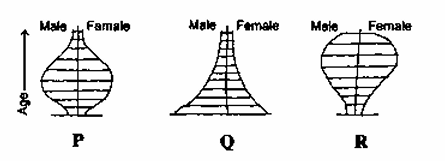
\includegraphics[width=0.6\textwidth]{Fig 7.png}
\caption{}
\label{fig:question40}
\end{figure}

Each of them implies a strong socio-economic characteristic as indicated below.

\begin{multicols}{2}
\begin{enumerate}
\item 1. Aging community
\item 2. Economically vibrant community
\item 3. Multi ethnic community
\item 4. Young community with high birth rate
\end{enumerate}
\end{multicols}

Identify the correct set out of the following
\begin{multicols}{2}
\begin{enumerate}
\item P - 4, Q - 3, R - 1
\item P - 2, Q - 4, R - 3
\item P - 2, Q - 4, R - 1
\item P - 4, Q - 2, R - 3
\end{enumerate}
\end{multicols}
\hfill (GATE AR 2010)

\item The correct requirements provided to seek permission from the local authority for constructing a small residential building are

P - Key Plan

Q - Site Plan

R - Zonal Plan

S - Building Plan

T - Power of Attorney

U - Ownership Title

V - Transport Plan

W - Drainage / Sewerage/ Water Supply Plan

X - Solid waste disposal plan
\begin{multicols}{4}
\begin{enumerate}
\item P, Q, R, S, W
\item P, Q, S, U, W
\item P, S, V, W, X
\item Q, S, T, V, X
\end{enumerate}
\end{multicols}
\hfill (GATE AR 2010)

\item Two commands P and Q, in AutoCAD are given below.

P: Current settings: Mode = TFIM, Radius = 0.0000

Select first object or [Polyfine/Radius/Trim/mUltiple]:

Q: (TFIM mode) Current chamfer Dist1 = 0.0000, Dist2 = 0.0000

Select first line or [Polyfine/Distance/Angle/Trim/Method/mUltiple]:

The above mentioned commands are used for
\begin{multicols}{2}
\begin{enumerate}
\item P: Trim and Q: Trim
\item P: Fillet and Q: Trim
\item P: Fillet and Q: Chamfer
\item P: Trim and Q: Chamfer
\end{enumerate}
\end{multicols}
\hfill (GATE AR 2010)

\item A 'T- beam slab' is cast and cured. The shuttering has to be removed. The right sequence for removal of shuttering is
\begin{enumerate}
\item Base of beam $\rightarrow$ Sides of beam $\rightarrow$ Base of slab $\rightarrow$ Vertical support under beam
\item Base of slab $\rightarrow$ Sides of beam $\rightarrow$ Base of beam $\rightarrow$ Vertical support under beam
\item Base of slab $\rightarrow$ Sides of beam $\rightarrow$ Vertical support under beam $\rightarrow$ Base of beam
\item Base of beam $\rightarrow$ Base of slab $\rightarrow$ Sides of beam $\rightarrow$ Vertical support under beam
\end{enumerate}
\hfill (GATE AR 2010)

\item Bioclimatic chart developed by Victor Olygay shows the relationship between
\begin{multicols}{2}
\begin{enumerate}
\item Temperature and Precipitation
\item Relative Humidity and Precipitation
\item Air Movement and Temperature
\item Temperature and Relative Humidity
\end{enumerate}
\end{multicols}
\hfill (GATE AR 2010)

\item In a display window of height $H = 8.66$ m, of a retail store, a luminaire of intensity $L$ is mounted at a distance $L = 5$ m away from the rear. Its light beam is cast at an angle of $45^\circ$ from the ceiling, as shown in the figure alongside.
\begin{figure}[H]
\centering
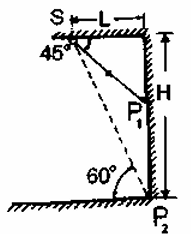
\includegraphics[width=0.3\textwidth]{Fig 8.png}
\caption{}
\label{fig:question45}
\end{figure}
The ratio of illumination at points $P_1$ and $P_2$ is
\begin{multicols}{4}
\begin{enumerate}
\item $1: \sqrt{3}$
\item $\sqrt{3}: 2$
\item $\sqrt{2}: 1$
\item $1: 2$
\end{enumerate}
\end{multicols}
\hfill (GATE AR 2010)

\item Following figure shows network for a particular project consisting of four activities.
\begin{figure}[H]
\centering
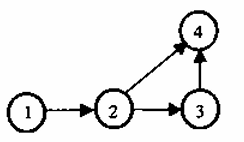
\includegraphics[width=0.3\textwidth]{Fig 9.png}
\caption{}
\label{fig:question46}
\end{figure}
Normal duration and crash time for each activity are given below.

\begin{table}[H]
\centering
\begin{tabular}{ccc}
\textbf{Activity} & \textbf{Normal duration}  & \textbf{Crash time} \\
& (in days) & (in days) \\
1 - 2 & 3 & 2 \\
2 - 3 & 4 & 2 \\
2 - 4 & 5 & 4 \\
3 - 4 & 7 & 5 \\
\end{tabular}
\end{table}

The minimum time required for completion of project is
\begin{multicols}{4}
\begin{enumerate}
\item 9 days
\item 13 days
\item 14 days
\item 19 days
\end{enumerate}
\end{multicols}
\hfill (GATE AR 2010)

\item Pick the \textbf{ODD} one from the figures given below with respect to Reflection and Transmission of light.

\begin{figure}[H]
\centering
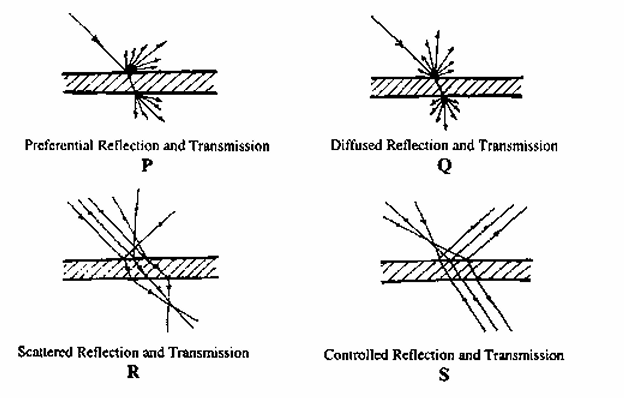
\includegraphics[width=0.8\textwidth]{Fig 10.png}
\caption{}
\label{fig:question47}
\end{figure}

\begin{multicols}{4}
\begin{enumerate}
\item P
\item Q
\item R
\item S
\end{enumerate}
\end{multicols}
\hfill (GATE AR 2010)

\textbf{Common Data for Questions}

\textbf{Common Data for Questions 48 and 49:}

A simply support beam PQ is subject to a load of 100 kN through a rigid link at the centre of the beam as shown in the figure below

\begin{figure}[H]
\centering
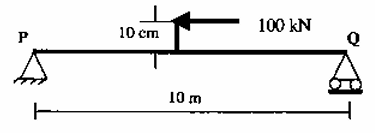
\includegraphics[width=0.6\textwidth]{Fig 11.png}
\caption{}
\label{fig:question48,49}
\end{figure}

\item Correct shear force diagram for the beam is
\begin{multicols}{2}
\begin{enumerate}
\item 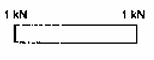
\includegraphics[width=0.3\textwidth]{Fig 12.png}
\item 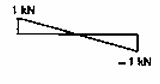
\includegraphics[width=0.3\textwidth]{Fig 13.png}
\item 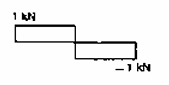
\includegraphics[width=0.3\textwidth]{Fig 14.png}
\item 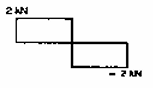
\includegraphics[width=0.3\textwidth]{Fig 15.png}
\end{enumerate}
\end{multicols}
\hfill (GATE AR 2010)

\item Bending moment diagram for the above beam is
\begin{multicols}{2}
\begin{enumerate}
\item 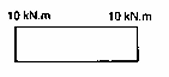
\includegraphics[width=0.3\textwidth]{Fig 16.png}
\item 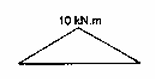
\includegraphics[width=0.3\textwidth]{Fig 17.png}
\item 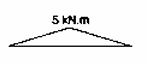
\includegraphics[width=0.3\textwidth]{Fig 18.png}
\item 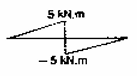
\includegraphics[width=0.3\textwidth]{Fig 19.png}
\end{enumerate}
\end{multicols}
\hfill (GATE AR 2010)

\textbf{Common Data for Questions 50 and 51:}

A plot of land is to be developed as a residential neighbourhood. The key development conditions and project requirements are given below

Plot area : 1.25 Hectares

Maximum permissible FAR : 350

Maximum permissible ground coverage : 30\%

Maximum permissible height : 45 m

Density of population : 800 ppHa

Average household size : 3.55

\begin{table}[H]
\centering
\begin{tabular}{ccc}
\textbf{Building Type} &\textbf{Percentage of Dwelling Units} & \textbf{Total Built up Area (in sq. m)} \\
L.I.G. & 20 & 4480 \\
M.I.G. & 55 & 18600 \\
H.I.G. & 25 & 14200 \\
\end{tabular}
\end{table}

\item The total number of dwelling units under L.I.G., M.I.G. and H.I.G. respectively, are

\begin{table}[H]
\centering
\begin{tabular}{|c|c|c|c|}
\hline
& L.I.G. & M.I.G & H.I.G. \\
\hline
P & 56 & 155 & 71 \\
\hline
Q & 60 & 142 & 71 \\
\hline
R & 56 & 150 & 63 \\
\hline
S & 59 & 155 & 63 \\
\hline
\end{tabular}
\end{table}

\begin{multicols}{4}
\begin{enumerate}
\item P
\item S
\item Q
\item R
\end{enumerate}
\end{multicols}
\hfill (GATE AR 2010)

\item With the above data, the covered area of each flat (in sq. m) under L.I.G., M.I.G. and H.I.G. respectively are

\begin{table}[H]
\centering
\begin{tabular}{|c|c|c|c|}
\hline
& L.I.G. & M.I.G & H.I.G. \\
\hline
P & 70 & 130 & 200 \\
\hline
Q & 80 & 120 & 200 \\
\hline
R & 70 & 130 & 220 \\
\hline
S & 80 & 120 & 220 \\
\hline
\end{tabular}
\end{table}

\begin{multicols}{4}
\begin{enumerate}
\item Q
\item S
\item R
\item P
\end{enumerate}
\end{multicols}
\hfill (GATE AR 2010)

\textbf{Linked Answer Questions}

\textbf{Statement for Linked Answer Questions 52 and 53:}

A person has purchased an old building at a cost of Rs. 2,50,000/-, excluding the cost of land. The scrap value of the building is 10 \% of the cost of purchase and the future life of the building is 20 years.

\item The total amount of sinking fund at the end of 20 years will be
\begin{multicols}{4}
\begin{enumerate}
\item Rs. 1,35,000/-
\item Rs. 1,90,000/-
\item Rs. 2,25,000/-
\item Rs. 2,30,000/-
\end{enumerate}
\end{multicols}
\hfill (GATE AR 2010)

\item If the rate of interest is 7 \%, then the annual installment of sinking fund will be
\begin{multicols}{4}
\begin{enumerate}
\item Rs. 4,583/-
\item Rs. 4,855/-
\item Rs. 5,507/-
\item Rs. 5,640/-
\end{enumerate}
\end{multicols}
\hfill (GATE AR 2010)

\textbf{Statement for Linked Answer Questions 54 and 55:}

A standpipe system in a 39 m tall building has a rooftop reservoir for fire fighting containing 1/2 hour water supply.

\item Assuming that each floor has one hose, the delivery rate (in litre per second) of the fire hose at greatest pressure is
\begin{multicols}{2}
\begin{enumerate}
\item 75
\item 78
\item 81
\item 84
\end{enumerate}
\end{multicols}
\hfill (GATE AR 2010)

\item The volume of water (in cubic metre) required for the reservoir is
\begin{multicols}{2}
\begin{enumerate}
\item 105
\item 110
\item 120
\item 130
\end{enumerate}
\end{multicols}
\hfill (GATE AR 2010)

\textbf{General Aptitude (GA) Questions}

\item 25 persons are in a room. 15 of them play hockey, 17 of them play football and 10 of them play both hockey and football. Then the number of persons playing neither hockey nor football is:
\begin{multicols}{4}
\begin{enumerate}
\item 2
\item 17
\item 13
\item 3
\end{enumerate}
\end{multicols}
\hfill (GATE AR 2010)

\item \textit{Choose the most appropriate word from the options given below to complete the following sentence:}

\textbf{If we manage to ------------ our natural resources, we would leave a better planet for our children.}

\begin{enumerate}
\item uphold
\item restrain
\item cherish
\item conserve
\end{enumerate}
\hfill (GATE AR 2010)

\item \textit{The question below consists of a pair of related words followed by four pairs of words. Select the pair that best expresses the relation in the original pair.}

\textbf{Unemployed : Worker}

\begin{enumerate}
\item fallow : land
\item unaware : sleeper
\item wit : jester
\item renovated : house
\end{enumerate}
\hfill (GATE AR 2010)

\item \textit{Which of the following options is the closest in meaning to the word below:}

\textbf{Circulious}

\begin{enumerate}
\item cyclic
\item indirect
\item confusing
\item crooked
\end{enumerate}
\hfill (GATE AR 2010)

\item \textit{Choose the most appropriate word from the options given below to complete the following sentence:}

\textbf{His rather casual remarks on politics ------------ his lack of seriousness about the subject.}

\begin{enumerate}
\item masked
\item belied
\item betrayed
\item suppressed
\end{enumerate}
\hfill (GATE AR 2010)

\item Hari (H), Gita (G), Irfan (I) and Saira (S) are siblings (i.e. brothers and sisters). All were born on 1st January. The age difference between any two successive siblings (that is born one after another) is less than 3 years. Given the following facts:


i.  Hari's age + Gita's age $>$ Irfan's age + Saira's age.

ii.  The age difference between Gita and Saira is 1 year. However, Gita is not the oldest and Saira is not the youngest.

iii.  There are no twins.

In what order were they born (oldest first)?

\begin{multicols}{4}
\begin{enumerate}
\item HSIG
\item SGHI
\item IGSH
\item IHSG
\end{enumerate}
\end{multicols}
\hfill (GATE AR 2010)

\item 5 skilled workers can build a wall in 20 days; 8 semi-skilled workers can build a wall in 25 days; 10 unskilled workers can build a wall in 30 days. If a team has 2 skilled, 6 semi-skilled and 5 unskilled workers, how long will it take to build the wall?
\begin{multicols}{4}
\begin{enumerate}
\item 20 days
\item 18 days
\item 16 days
\item 15 days
\end{enumerate}
\end{multicols}
\hfill (GATE AR 2010)

\item \textbf{Modern warfare has changed from large scale clashes of armies to suppression of civilian populations. Chemical agents that do their work silently appear to be suited to such warfare; and regretfully, there exist people in military establishments who think that chemical agents are useful tools for their cause.}

\textit{Which of the following statements best sums up the meaning of the above passage:}

\begin{enumerate}
\item Modern warfare has resulted in civil strife.
\item Chemical agents are useful in modern warfare.
\item Use of chemical agents in warfare would be undesirable.
\item People in military establishments like to use chemical agents in war.
\end{enumerate}
\hfill (GATE AR 2010)

\item Given digits 2, 2, 3, 3, 3, 4, 4, 4, 4 how many distinct 4 digit numbers greater than 3000 can be formed?
\begin{multicols}{4}
\begin{enumerate}
\item 50
\item 51
\item 52
\item 54
\end{enumerate}
\end{multicols}
\hfill (GATE AR 2010)

\item If $137 + 276 = 435$ how much is $731 + 672$?
\begin{multicols}{4}
\begin{enumerate}
\item 534
\item 1403
\item 1623
\item 1513
\end{enumerate}
\end{multicols}
\hfill (GATE AR 2010)

\end{enumerate}
\end{document}